\chapter{Literature Review}
\section{Introduction}


% we need this in the preamble

% \usepackage{tikz}
% \usetikzlibrary{shapes.geometric, arrows.meta, positioning}
% \tikzstyle{process} = [rectangle, rounded corners, minimum width=5.5cm, minimum height=1.2cm,text centered, draw=black, fill=blue!10]
% \tikzstyle{arrow} = [thick,->,>=stealth]



 


\lipsum[1]


\section{Some Section}

\lipsum[1] 

\textcolor{red}{This is how you insert an image by referencing it like this:} Figure \ref{fig:encoder-only} shows XYZ.
 

\begin{figure}[H]
    \centering
    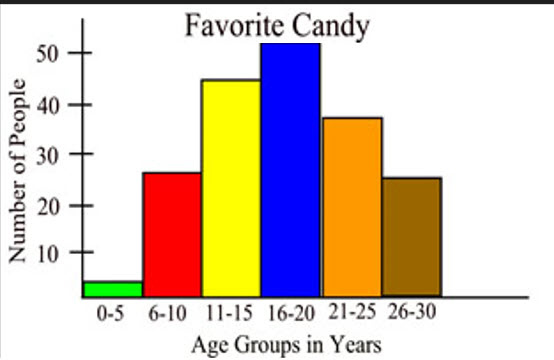
\includegraphics[width=0.6\textwidth]{figures/chap2_fig/histogram1.jpg}
    \captionsetup{
    labelfont={bf,it}, 
    textfont=it,  
    }
    \caption{Histogram of XYZ}
    \label{fig:encoder-only}
\end{figure}

\lipsum[1]

\subsection{Subsection 1}
\lipsum[1]
 
\textcolor{red}{This is how to enter an equation and reference it. Equation \ref{eqn:pos1} and \ref{eqn:pos1} show how XYZ is implemented.
}

\begin{equation}
\label{eqn:pos1}
    TE_{(pos,2i)}=sin(pos/23^{2i/Lm})
\end{equation}

\begin{equation}
\label{eqn:pos2}
    KN_{(pos,2i+1)}=cos(pos/453^{2i/Lm})
\end{equation}
 
\lipsum[1]

  

\section{Another Section}

 
\lipsum[1]

\textcolor{red}{This is the correct format for a table, including the caption and proper alignment (centered and italicized).}

\begin{table}[H]
\centering
\captionsetup{
    labelfont=bf, 
    textfont=it,  
    justification=centering
}
\caption{My Table About Something}
\label{tab:sampling-techniques}
\begin{tabularx}{\textwidth}{@{}X X@{}}
\toprule
\rowcolor[gray]{0.95} % Lighter shade for subtlety
\textbf{Reference} & \textbf{Technique} \\
\midrule
something here & Technique here \\
something here & Technique here\\
something here  & Technique here \\
something here  & Technique here\\
something here  & Technique here \\
\bottomrule
\end{tabularx}
\end{table}
 

\subsection{Subsection}
 
\lipsum[1]
 
\subsection{Subsection}
\lipsum[1]
 
 
\subsubsection{Sub subsection}
 
\lipsum[1]

 
 
\section{Summary}

\lipsum[1]